
\documentclass[12pt]{article}

\usepackage{graphicx}
\graphicspath{ {./images/} }

\usepackage{epsfig}
\usepackage{amsmath,amsthm}
\usepackage{listings}


\newtheorem{lemma}{Lemma}
\newtheorem{theorem}{Theorem}


\usepackage{titlesec}
\titleformat{\section}
{\normalfont\Large\bfseries}{Question~\thesection:}{1em}{}

\newlength{\toppush}
\setlength{\toppush}{2\headheight}
\addtolength{\toppush}{\headsep}


\def\subjnum{Comp 160}
\def\subjname{Algorithms}


\def\doheading#1#2#3{\vfill\eject\vspace*{-\toppush}%
  \vbox{\hbox to\textwidth{{\bf} \subjnum: \subjname \hfil Erli Cai}%
    \hbox to\textwidth{{\bf} Tufts University, Fall 2020 \hfil#3\strut}%
    \hrule}}


\newcommand{\htitle}[1]{\vspace*{1.25ex plus 1ex minus 0ex}%
\begin{center}
{\large\bf #1}
\end{center}} 



\begin{document}
\doheading{2}{title}{Homework 00}
\setlength\parindent{0pt}
\section{Context Free Pumping Lemma}
$A_P = {a^nb^mc^r | n \times m = r}$\\
Assuming $A_P$ is context free, then context free pumping lemma should apply to $A_P$\\
For any length $p > 0$,
we can have a string $w = a^pb^pc^{p^2}$\\
Writing w = uvxyz where $|vxy| \le p$ and $|vy| > 0$\\
Then we will have the following cases:\\
1) vxy are all a's or all b's or all c's. Then $uv^2xy^2z$ adds only one of them it is not in $A_P$. This contradict to pumping lemma (which says it should be in $A_P$)
2) vxy have some a's and some b's. Then  $uv^2xy^2z$ only add a's and b's but not any c. So it is not in $A_P$(which says it should be in $A_P)$.\\
3) vxy have some c's and some b's.\\  
Assuming v,y has m b's and n c's. Then $uv^2xy^2z = a^pb^{p+m}c^{p^2+n}$. If $m \ge 1$, then n = p and $|vy| \ge p+1$ contradict to our assumption $|vxy| \le p$. If m =0, then n = 0, then $|vy| = 0$ contradicts to our assumption assumption that $|vy| > 0$. \\

In all three cases, we have contradiction. So our assumption that $A_P$ is context free is not true.

\pagebreak



\section{CFG’s from Regular Expressions}
Regular expressions can be built inductively from 3 atomic element and 3 composite expressions. So we only need to prove we can create CFG for each one of them.\\
Atomic elements:\\
1) a, corresponding CFG: $S\rightarrow a$\\
2) $\epsilon$ corresponding CFG: $S\rightarrow \epsilon$\\
3) $\emptyset$ corresponding CFG: $S$\\

Composite elements: Assuming now $R_1$ and $R_2$ are regular languages whose corresponding CFG are A and B\\
1) $R_1 \cup R_2$, corresponding CFG: $S \rightarrow A|B$

2) $R_1R_2$, corresponding CFG: $S \rightarrow AB$

3) $R_1^*$, corresponding CFG:  $S \rightarrow AS|\epsilon$\\

we can use these to build a CFG for any regular expressions correspondingly.
\pagebreak


\section{Pushdown Automata}

Pushdown Automata $M = (Q,\Sigma,\Gamma, \delta, s, F)$\\
Q = {q1,q2,q3,q4,q5}\\
$\Sigma = \{a,b\}$\\
$\Gamma = \{A,B,\$\}$\\
s = q1\\
$F = \{q5\}$

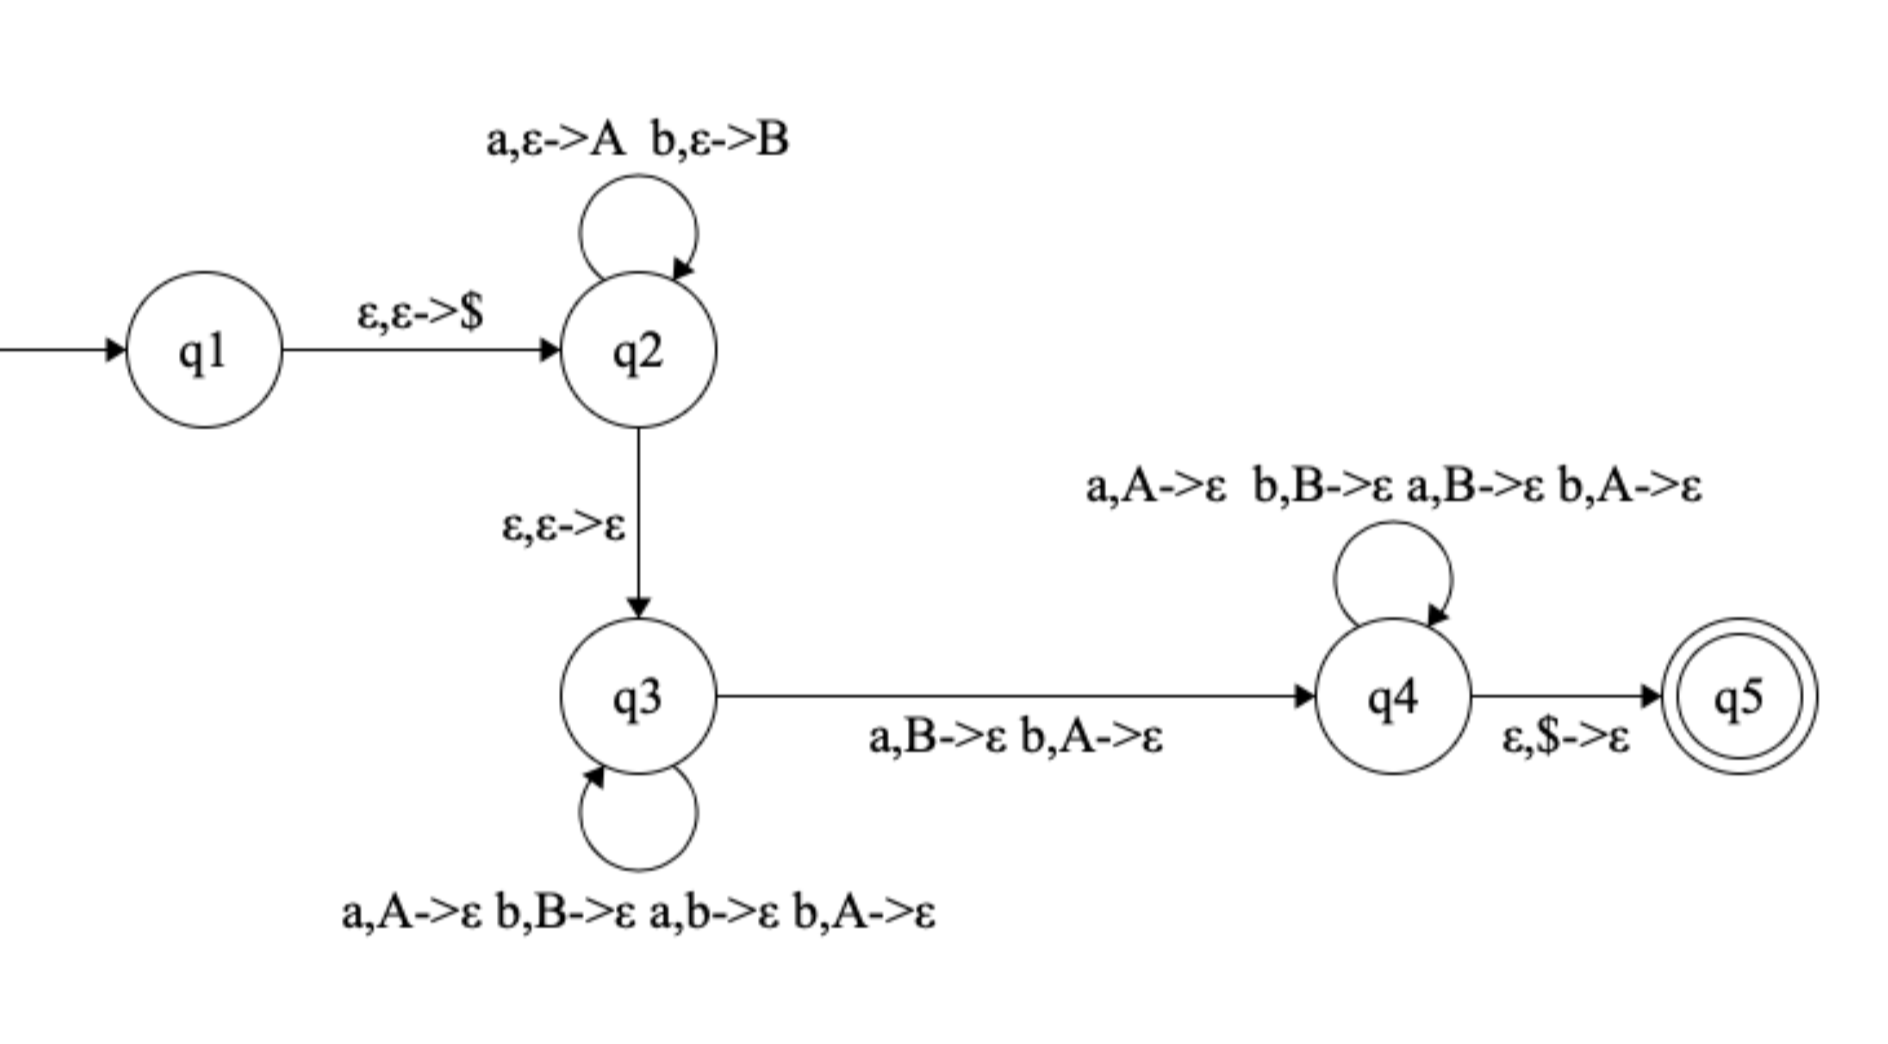
\includegraphics[scale = 0.3]{2}


A palindromic string of even length is symmetric from middle. Therefore, a non palindromic string would have at least one different character on each sides of middle and same distance from middle so it breaks this symmetry. Transition from q3 to q4 ensures at least one such difference.













\end{document}


